\section{RandAO Protocol}\label{sec:protocol}

\subsection{Overview}\label{sec:protocol_overview}

The RandAO protocol builds upon the commit-reveal scheme discussed in Section~\ref{sec:related_work_commit_reveal}, replacing hash commitments with time-lock puzzles (Section~\ref{sec:timelock}). A set of validators $\mathcal{V} = \{v_1, \ldots, v_n\}$ produces a value per \emph{round}; every pending request is bound to a round and receives its own value derived from the round's output.

\begin{figure}[H]
\centering
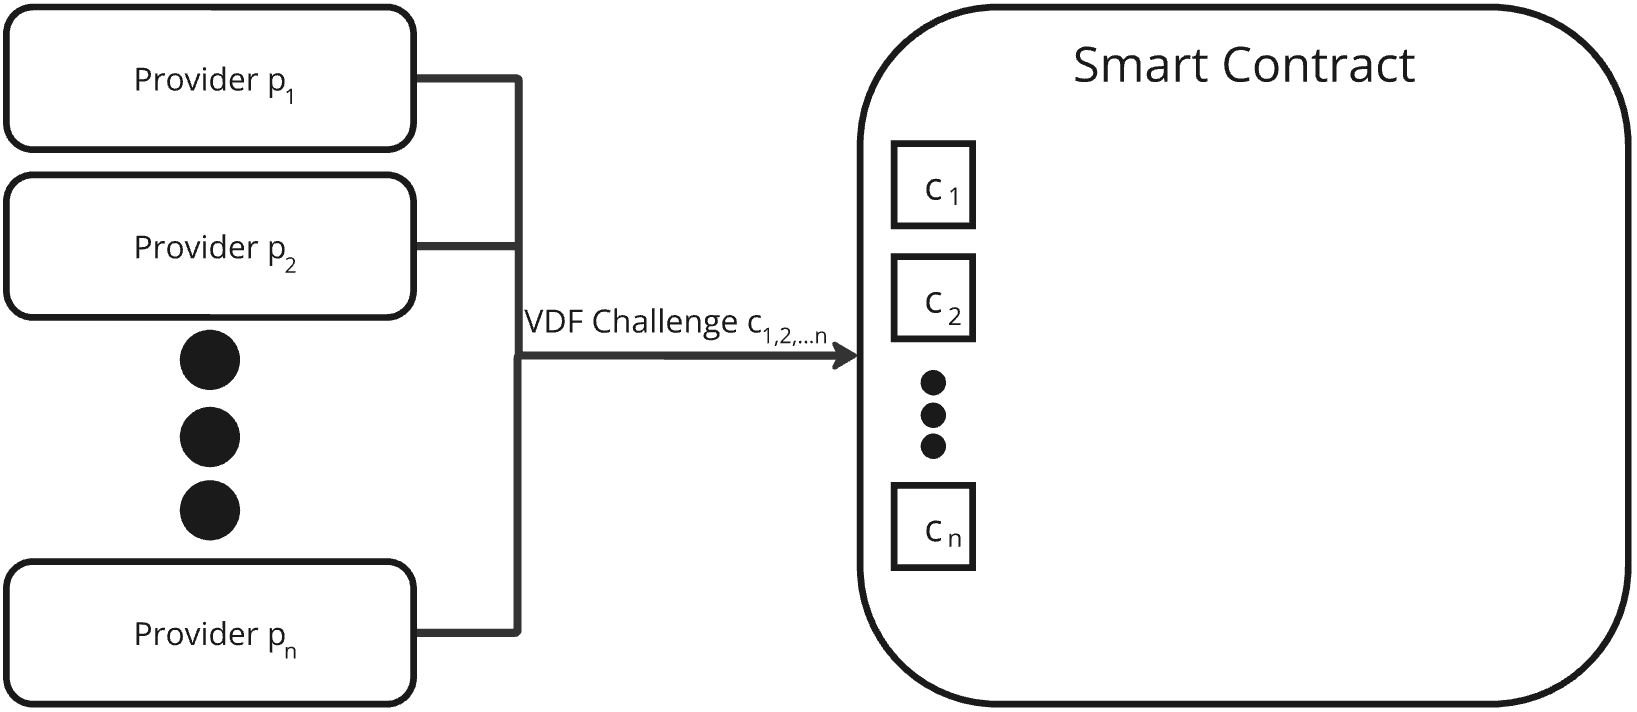
\includegraphics[width=0.8\textwidth]{images/protocol_commitment_phase.png}
\caption{Commitment: every validator posts its puzzle to the beacon process before the window closes}
\label{fig:protocol_commitment}
\end{figure}

\subsection{Puzzles}\label{sec:puzzles}

Each validator prepares RSA moduli ahead of time, $N = p \cdot q$ with $p$ and $q$ random primes of 1024 bits. Generating a 1024-bit prime takes about 18~ms on a commodity CPU, so a validator keeps a small pool. A modulus is used for exactly one round.

The puzzle input is not chosen by the validator; it is fixed by the round:
\begin{align*}
    \text{seed} &= \text{beacon} \,\|\, r \,\|\, v_i \\
    x &= \big(\text{expand}(\text{seed}) \bmod N\big)^2 \bmod N
\end{align*}
where $\text{expand}$ stretches the seed with SHA-256 to the size of $N$ plus 64 bits. The validator's contribution to round $r$ is
\begin{equation}
    y_i = x^{2^T} \bmod N ,
\end{equation}
which it computes instantly with its trapdoor (39~ms in Node.js at 2048 bits and $T = 2^{27}$) and which anyone else can compute only through $T$ sequential squarings.

\subsection{Round}\label{sec:round}

A round opens when requests are waiting. Requests bind to the open round until its first commitment; later requests wait for the next round.

\begin{enumerate}
    \item \textbf{Commit}: Each active validator posts its modulus $N_i$. The first commitment starts a commitment window of length $W$; commitments after the window are refused. Because $x$ is fixed by the round, posting $N_i$ fixes $y_i$.

    \item \textbf{Reveal}: Each committed validator posts $y_i$ together with one factor $p_i$ of $N_i$. The beacon checks the reveal through the \texttt{timelock@1.0} device: $1 < p_i < N_i$, $p_i \mid N_i$, and
    \begin{equation}
        y_i = x^{\,2^T \bmod (p_i-1)(q_i-1)} \bmod N_i .
    \end{equation}
    Publishing the factor is safe because the modulus is never used again.

    \item \textbf{Crack}: If a committed validator has not revealed by the reveal deadline, any validator may compute its $y_i$ by sequential squaring and post it with a Wesolowski proof (Section~\ref{sec:vdf}), which the device checks. The cracker earns the withholder's fee for the round, and the withholder receives a strike.

    \item \textbf{Aggregation}: When every committed $y_i$ is known, the round value is
    \begin{equation}
        V_r = \text{SHA-256}\big(\texttt{"rng/timelock"} \,\|\, \text{beacon} \,\|\, r \,\|\, y_{1} \,\|\, \cdots \,\|\, y_{k}\big)
    \end{equation}
    with the contributions ordered by validator address, and each request receives $\text{SHA-256}(V_r \,\|\, \text{requestId})$.
\end{enumerate}

If fewer than a minimum number of validators commit, the round is void and its requests move to the next round. The beacon stores every round's commitments, reveals, cracks and value, so anyone can re-verify any result.

\subsection{Any-Honest Security}\label{sec:any_honest}

Suppose validator $v_h$ is honest. When the commitment window closes, $y_h$ is fixed, but nobody except $v_h$ can compute it before $T$ sequential squarings, which by construction take longer than the window even on an attacker's fastest hardware. A dishonest validator deciding whether to commit therefore cannot know the round's value, and a dishonest validator deciding whether to reveal cannot change it, since its own $y_i$ is fixed and recoverable by cracking. The output is unpredictable and unbiasable unless every committed validator colludes.

\begin{figure}[H]
\centering
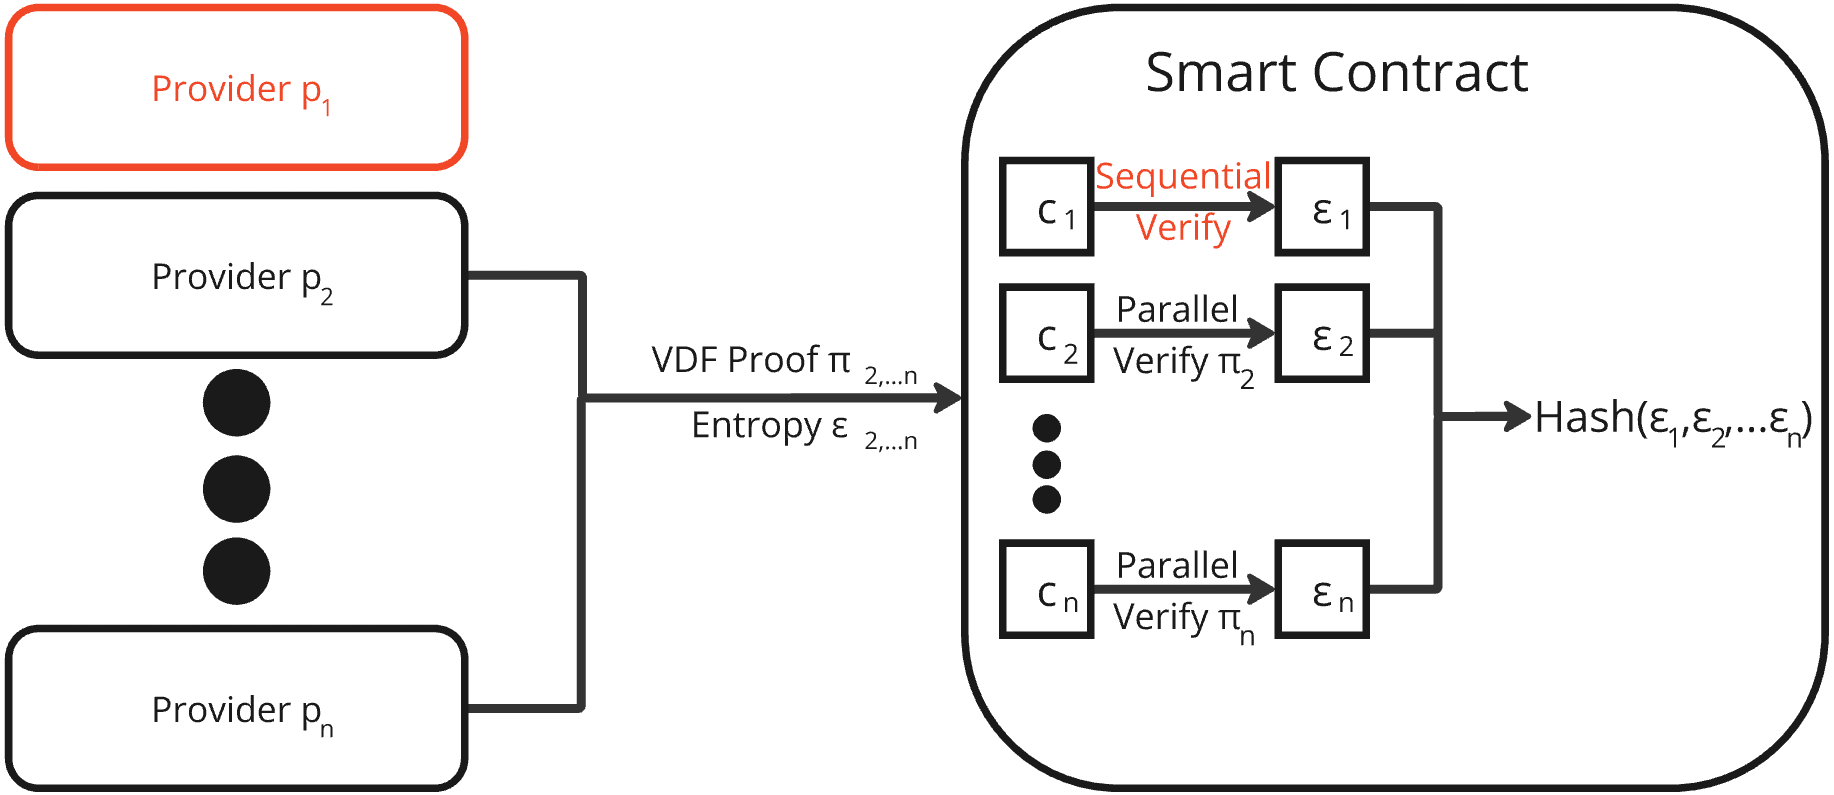
\includegraphics[width=0.8\textwidth]{images/verify-malicious-case.png}
\caption{A withholding validator cannot abort the round: its contribution is recovered by sequential computation from its commitment}
\label{fig:verify_malicious}
\end{figure}

\subsection{Timing}\label{sec:timing}

The parameters that set the protocol's timing are the number of squarings $T$, the commitment window $W$ and the reveal window $R$. Security requires
\begin{equation}
    \tau = \frac{T}{s_{\max}} > W ,
\end{equation}
where $s_{\max}$ is the squaring rate of the fastest hardware an attacker may own. The default $T = 2^{27}$ against an assumed $s_{\max}$ of $10^{7}$ squarings per second (ten times a fast CPU) gives $\tau \geq 13$~s against $W = 3$~s.

\subsubsection{Case: Standard}
Commitments arrive within the window, reveals follow immediately, and each reveal is checked with one exponentiation. A round costs two messages per validator and completes in a few seconds; requests that arrive while a round runs are batched into the next one.

\subsubsection{Case: A Validator Withholds}
The remaining validators wait until the reveal deadline and crack the missing puzzle. Native squaring runs at roughly one step per microsecond, so cracking and proving take a few minutes; JavaScript runs at about 14~$\mu$s per step and is only a fallback. The round is delayed, never changed.

\subsection{Validators}\label{sec:validators}

Validators are kept in a set by the beacon and are added or removed by the protocol's administrator, effective from the next round. Each validator signs its messages with its own wallet and generates its own puzzles; validators share no secret and need no key ceremony. A missed commitment or a cracked reveal is a strike; a validator with three strikes in a hundred rounds is suspended until reinstated, and a suspended validator neither commits nor earns. Opening the set to outside operators is planned once the protocol has run in production.

\subsection{Verification on the Node}\label{sec:device}

Our first version verified Pietrzak checkpoints by splitting each proof across a fleet of verifier processes, which cost dozens of messages per request. In the second version every check runs inside the node through the \texttt{timelock@1.0} HyperBEAM device. A reveal costs one modular exponentiation and a crack two short ones. The device is stateless and deterministic, so every node that computes or replays the beacon reaches the same verdict.
